\chapter{La paroi cellulaire : composition chimique et structure}\label{paroi}

\begin{abstract}
Dans ce chapitre, nous présentons la structure hiérarchique du matériau bois, de l'échelle de la molécule à celle de la pièce de bois. Bien qu'il s'agisse d'un matériau complexe et variable, le bois n'est constitué en grande majorité que de trois types d'atomes, soit l'hydrogène, le carbone et l'oxygène. Ces atomes se groupent ensuite en trois grands types de molécules aux propriétés physico-mécaniques distinctes, soit la cellulose, les hémicelluloses et la lignine. Les chaînes de cellulose s'assemblent en cristallites, puis en microfibrilles qui, imprégnées dans une matrice de cellulose et d'hémicelluloses, forment ensuite la paroi cellulaire.
\end{abstract}

\minitoc

\section{Composantes chimiques de la paroi cellulaire}

Le bois est constitué de trois composantes principales :

\begin{description}
\item[La cellulose] qui donne au bois la majeure partie de sa résistance mécanique
\item[Les hémicelluloses] qui constituent la matrice dans laquelle on retrouve la cellulose
\item[La lignine] qui permet de \og coller \fg les cellules du bois entre-elles. 
\end{description} 

En plus de ces principaux constituants, on retrouve une quantité variable de composés organiques de faible poids moléculaire appelés \textbf{extractibles} pouvant se loger dans la paroi cellulaire et en réduire l'hygroscopicité et la perméabilité en plus d'affecter la couleur du bois et sa résistance aux champignons de dégradation. Des \textbf{constituants inorganiques} ou \textbf{cendres} sont également présents dans des proportions faibles variant de 0,1\% à 0,5\% de la masse anhydre. Le Tableau \ref{tab:composes} présente la composition chimique de la paroi cellulaire.\\

\begin{table}[!h]
\centering
	\begin{tabular}{l c c}
	\hline
	& \bf Résineux & \bf Feuillus \\
	\hline
	\hline
	Cellulose & 40 - 50 & 40 - 50 \\
	Hémicelluloses & 20 - 30 & 25 - 40 \\
	Lignine & 25 - 35 & 20 - 25 \\
	Extractibles &	0 - 25 & 0 -25 \\
	\hline
	\end{tabular}
\caption{Composition chimique de la paroi cellulaire du bois en proportion massique anhydre de la paroi cellulaire (\%) (adapté de \cite{choong1997wood})}
\label{tab:composes}
\end{table}

On qualifie souvent le bois de polymère car il est constitué de plusieurs composantes qui sont elles mêmes des polymères, c'est-à-dire des substances constituées par de grandes molécules formées par la répétition de plus petites unités structurales. Les polymères constituant la paroi cellulaire sont mélangés de façon ordonnée, cette organisation lui conférant ses propriétés mécaniques et par le fait même celles du bois.

\subsection{Cellulose}

La cellulose est la composante la plus importante du bois, autant en pourcentage de la masse anhydre que d'effet sur les propriétés mécaniques et l'hygroscopicité du bois. La cellulose est un polymère fibreux très stable chimiquement. Il est donc difficile de la modifier artificiellement pour en changer les propriétés. Il est aussi difficile d'isoler la cellulose pure car elle est étroitement liée avec d'autres polysaccharides, les hémicelluloses.\\

La cellulose (Figure \ref{fig:cellulose}) est un polymère contenant des molécules de longueurs différentes constituées d'une répétition de monomère appelés cellobiose. La cellobiose est l'unité de base de la cellulose et est constituée de deux cycles de glucose liés par des liaisons $\beta$-glycosidiques lui conférant ses propriétés structurales.\\


Chaque unité de cellobiose fait environ 1,03 nm de longueur et a des dimensions transversales de 0,84 x 0,79 nm dans les portions cristallines de la cellulose. Le degré de polymérisation de la cellulose, c'est-à-dire le nombre d'unités de glucose que l'on retrouve dans une molécule de cellulose, est d'environ \numprint{10000} dans la paroi secondaire des cellules du bois. Ceci correspond à une longueur moyenne de 5 \micro m pour la molécule de cellulose du bois.

\begin{figure}[h]
\centering
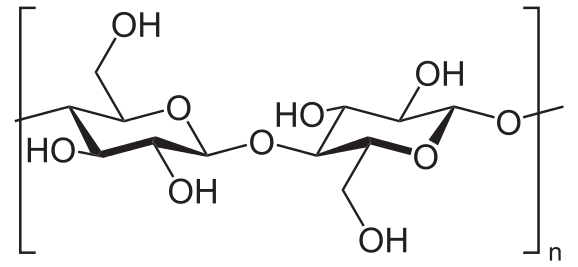
\includegraphics[scale=0.3]{img/cellulose}
\caption{La cellulose est un polymère monotone de cellobiose}
\label{fig:cellulose}
\end{figure}

La cellulose se présente sous forme cristalline dans les parois cellulaires, mais des zones amorphes sont aussi présentes. La cristallinité est une propiété d'un solide dont les constituants primaires sont disposés selon un motif régulier répété un grand nombre de fois. Les parties amorphes sont donc moins \og organisées \fg, ce qui leur confère de moins bonnes propriétés mécaniques et une plus grande hygroscopicité. 

Voici quelques faits saillant pour décrire la molécule de cellulose :

\begin{enumerate}
\item La molécule de cellulose a une forme rubanée,

\marginpar{L'amylase, le polymère de glucoses liés par des laisons $\alpha$ est une molécule de réserves énergétiques qui n'a pas de propriétés mécaniques}
\item les liaisons $\beta$-glycosidique donnent à la chaîne de cellulose une grande résistance mécanique. 

\item de nombreux groupements hydroxyles (--OH) sont disponibles le long de la chaîne de cellulose pour former des liaisons hydrogène latérales avec d'autres chaînes de cellulose tel qu'illustré à la Figure \ref{fig:cellulose_hydrogene}.\\
\end{enumerate}

Rappelons qu'une liaison hydrogène est de nature électrostatique. C'est une force intermoléculaire impliquant un atome d'hydrogène et un atome électronégatif comme l'oxygène. Ce sont également les groupements hydroxyles disponibles le long de la chaîne de cellulose qui en expliquent l'hygroscopicité.

% c'est faux
% et qu'elle consiste en la mise en commun d'un électron entre l'atome d'oxygène et l'atome d'hydrogène.
% Oui, t'as raison. Je le disais aux étudiant que c'était faux, mais je n'avais jamais pris le temps de le corriger. 

\begin{figure}[h]
\centering
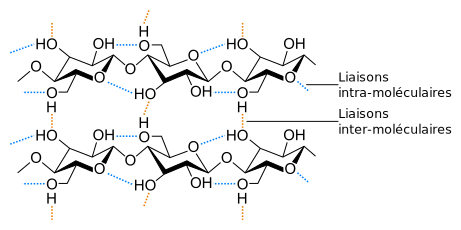
\includegraphics[scale=0.8]{img/ch6_cellulose_hydrogene}
\caption{Liaisons hydrogène inter-moléculaires et intra-moléculaires entre deux molécules de cellulose}
\label{fig:cellulose_hydrogene}
\end{figure}

\subsection{Hémicelluloses}

% c'est faux
% Les hémicelluloses sont des polysaccharides  de composition semblable à la cellulose 
% AA: je pense qu'on devrait dires combien de C ont chacun des monomères décrits ici. 
Les hémicelluloses sont des polysaccharides de masse moléculaire beaucoup plus faible que la cellulose. Les monomères de l'hémicellulose peuvent être du xylose, du mannose, du galactose, du rhamnose ou de l'arabinose liée par des liaisons $\alpha$ ou $\beta$. Ils constituent de 20 à 35\% de la masse anhydre du bois et sont solubles dans les bases faibles et facilement hydrolysables dans les acides faibles pour former des sucres et des acides uroniques. Un groupe d'hémicelluloses appelés xylanes est dominant chez les feuillus et un autre groupe appelé glucomannanes est dominant chez les résineux.

\subsection{Lignine}

% Ce paragraphe est d'une complexité extraordinaire ! Tout tombe comme un cheveux sur la soupe. C'est quoi un procédé d'extraction ? C'est quoi la fraction remanente ? C'est quoi la lignine de Klason ? 
% AA; Ok, voilà qui est mieux je pense.
La lignine n'est formée que dans les parois cellulaires des plantes vivantes des spermatophytes, des ptéridophytes et des mousses. Le mot lignine vient du latin \textit{lignum} pour bois. On définit la lignine naturelle présente dans le bois comme un polymère tridimensionnel amorphe appelé protolignine produit dans la zone cambiale.\\

La lignine, quant à elle, réfère à la molécule que l'on peut extraire du bois à l'aide d'un procédé chimique (les plus connus sont les procédés Soda, sulfite et Kraft) ou thermique (pyrolyse). La distinction entre les termes lignine et protolignine vient du fait que les différent procédés d'extraction applicables altèrent la structure de la molécule. Il faut donc spécifier le procédé d'extraction utilisé lorsqu'on parle de lignine. Par exemple, suite à l'extraction à partir d'acides minéraux forts, on obtient la lignine dite \og de Klason \fg dont la structure générale est illustrée à la Figure~\ref{fig:lignine}. Elle consiste en un arrangement tridimensionnel complexe de noyaux phénoliques. Plusieurs groupements hydroxyles sont présents, ce qui résulte en une certaine hygroscopicité qui demeure tout de même bien inférieure à celle de la cellulose. On dit d'ailleurs que la lignine est \og partiellement hydrophobe \fg. La structure de la protolignine est légèrement différente de celle présentée à la Figure~\ref{fig:lignine} mais la structure générale est similaire. Il est aussi reconnu que la protolignine ne constitue pas un seul composé chimique mais un groupe de composés. La protolignine est différente entre les feuillus et les résineux et même entre les différentes espèces de feuillus et de résineux.\\

La protolignine est rigide mais remarquablement thermoplastique ou viscoélastique (Figure~\ref{fig:contrainte}), ce qui confère au bois la même propriété qui est exploitée dans le procédé de pressage à chaud des panneaux agglomérés à base de bois (180\textdegree C < T < 220\textdegree C) et lors du séchage à haute température (T > 100\textdegree C). Elle est produite dans la zone cambiale et est présente dans les cavités fines de la paroi cellulaire contribuant à en réduire l'hygroscopicité. La protolignine n'est pas distribuée uniformément dans la paroi cellulaire. On retrouve jusqu'à 70\% (base anhydre) de protolignine dans la lamelle moyenne composée entre les cellules. Cette proportion s'abaisse rapidement jusqu'à environ 10\% dans la paroi secondaire. Inversement, la teneur en cellulose est faible dans la lamelle moyenne composée et élevée dans la paroi secondaire.

\begin{figure}[h]
\centering
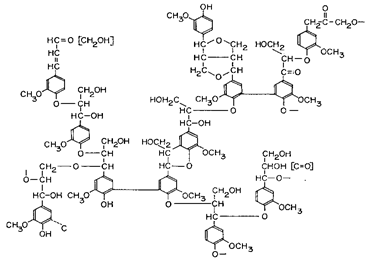
\includegraphics[scale=0.8]{img/ch6_lignine}
\caption{Description schématique de la structure de la lignine de Klason (d'après \cite{choong1997wood}).}
\label{fig:lignine}
\end{figure}

\begin{figure}[h]
\centering
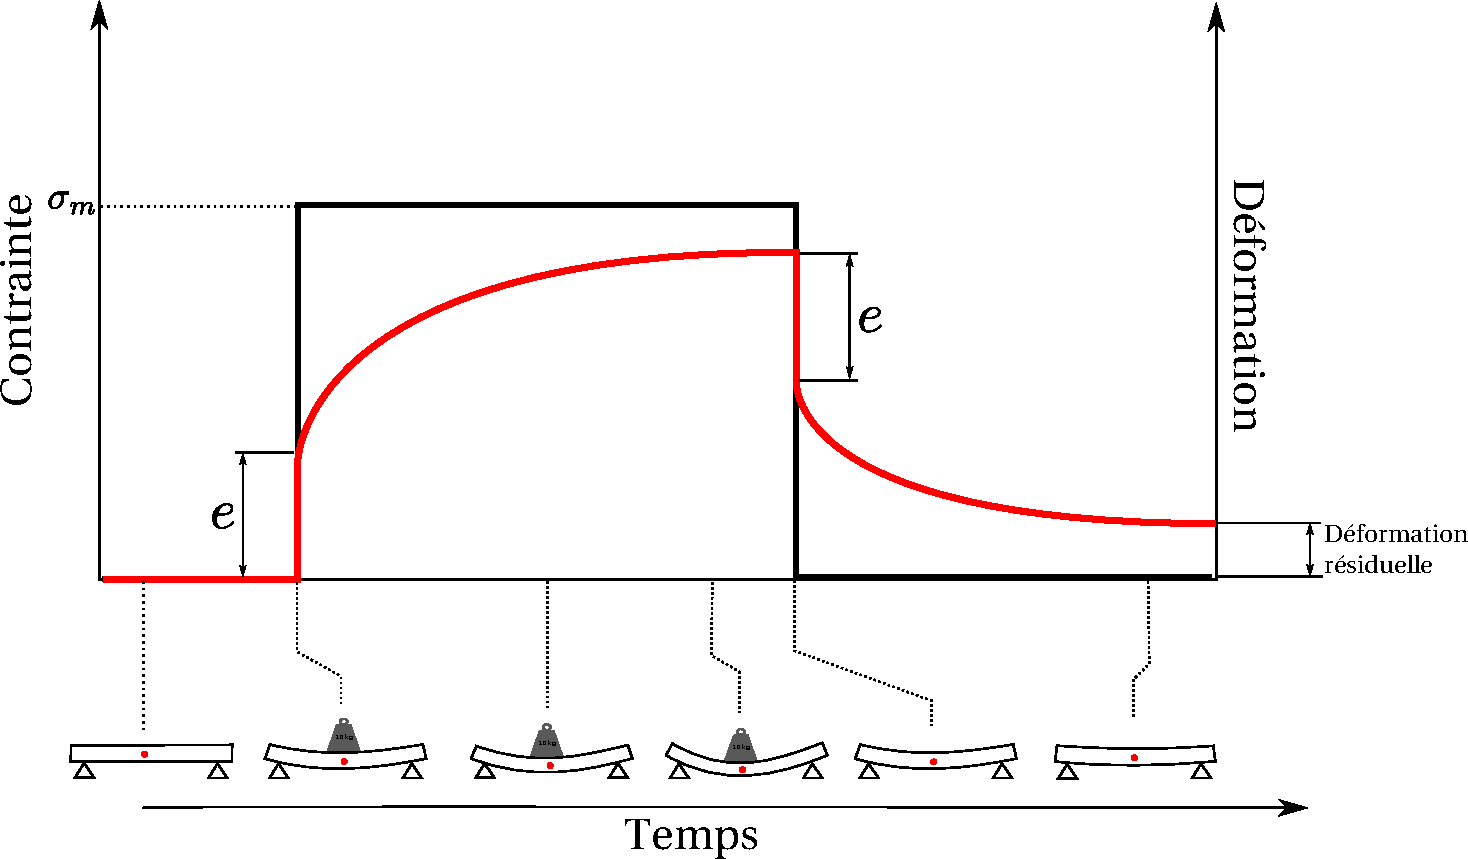
\includegraphics[scale=0.5]{img/ch6_contrainte}
\caption{Viscoélasticité du bois due aux propriétés de la cellulose (composante élastique) et aux propriétés de la lignine (composante visqueuse).}
\label{fig:contrainte}
\end{figure}

\subsection{Substances extractibles}

Les substances extractibles peuvent être infiltrées dans les parois cellulaires ou déposées à la surface des lumens. Elles sont solubles dans l'eau chaude et/ou dans des solvants organiques (alcool, benzène). Les extractibles ne représentent généralement qu'une faible proportion de la masse anhydre du bois. Toutefois, ils peuvent représenter jusqu'à 35\% de la masse anhydre chez certains bois dont le quebracho \textit{(Schinopsis lorentzii Engl.}) très riche en tannin utilisé comme adhésif dans l'industrie des panneaux composites à base de bois dans quelques usines d'Amérique du Sud.\\

Les extractibles représentent une large gamme de composés organiques dont les polyphénols (ex. tannins) et les oléorésines (ex. térébenthine) sont les plus importants. On y retrouve aussi des gommes, graisses, acides gras, cires et hydrocarbures volatils. Ces produits sont responsables de plusieurs propriétés du bois dont l'odeur et la couleur du bois de duramen, la résistance aux champignons de pourriture et aux insectes, la perméabilité et la masse volumique. Comme les extractibles ne sont pas hygroscopiques, ils réduisent l'hygroscopicité du bois lorsqu'ils sont présents en forte proportion.

\subsection{Cendres}

Les cendres sont des composées inorganiques représentant environ 0,1 à 0,5\% de la masse anhydre du bois. On y retrouve principalement des composés à base de calcium, potassium, et magnésium. Le manganèse peut aussi être présent. Il est la cause des taches minérales chez les érables durs. La silice peut compter jusqu'à 2\% de la masse anhydre chez certaines espèces. Elle cause de graves problèmes d'usure prématurée des outils de coupe.

\section{Structure de la paroi cellulaire}

La paroi cellulaire est formée de structures rubanées appelées microfibrilles incrustées dans la lignine amorphe pour former une paroi cellulaire rigide. La structure des composantes de la paroi cellulaire sera décrite ci-dessous.

\begin{figure}[h]
\centering
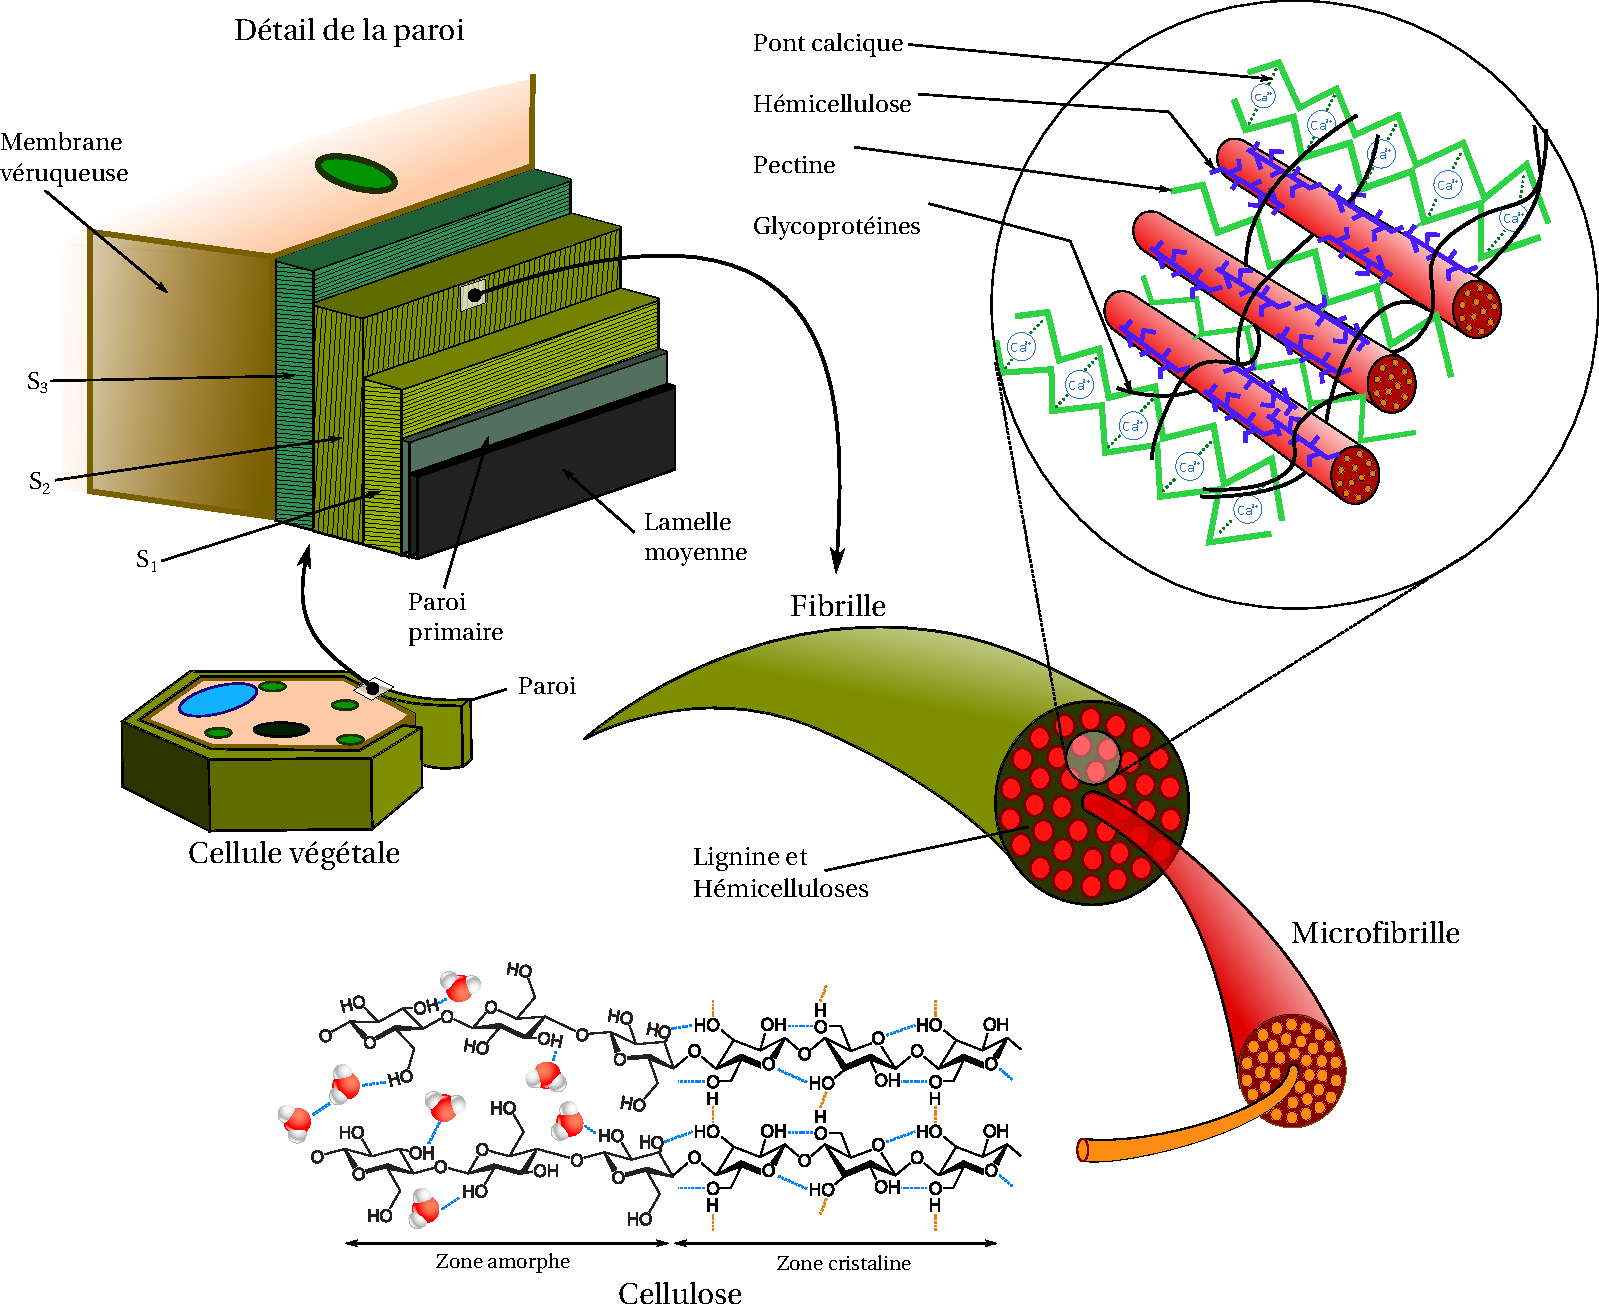
\includegraphics[scale=0.55]{img/ch6_cellule}
\caption{Schéma bilan regroupant l'ensemble des éléments du chapitre}
\label{fig:grosschema}
\end{figure}

\subsection{Structure des microfibrilles}

Les microfibrilles sont des bandes ou rubans de polysaccharides visibles au microscope électronique. Elles sont souvent présentées comme les constituants de base de la paroi cellulaire, ce qui n'est pas tout à fait exact. En fait, on peut séparer les microfibrilles en unités appelées cristallites, qui font environ 60 nm de longueur et 3,5 $\times$ 10 nm en section transversale tel qu'illustré à la Figure \ref{fig:grosschema}. Chaque cristallite contient environ 50 chaînes de cellulose juxtaposées. Le terme cristallite réfère au fait qu'il s'agit d'une unité critalline de molécules de cellobiose agencées de manière régulière grâce aux liaisons hydrogène latérales entre les chaînes de cellulose.\\

On retrouve également des régions amorphes où les chaînes de cellulose ne sont pas liées par des liaisons hydrogène latérales. Ces régions amorphes sont donc les sites disponibles pour l\textbf{'eau liée} puisque des groupements hydroxyles libres sont présents. La sorption de l'eau liée dans les régions amorphes force les chaînes de cellulose à s'éloigner les unes des autres, ce qui résulte en un \textbf{gonflement de la paroi cellulaire}.


\subsection{Groupement des microfibrilles}

Les microfibrilles sont constituées de 3 à 25 cristallites formant une structure fibreuse. Les microfibrilles sont organisées entre elles en lamelles superposées dans une matrice de lignine et d'hémicellulose (Figure \ref{fig:grosschema}). Elles sont déposées à angle variable pour former la paroi cellulaire. Cette structure est analogue à celle du béton armé sauf qu'ici, la matrice est plastique. La grande élasticité de la cellulose pour des charges à court terme et la plasticité de la lignine pour des charges à long terme expliquent le comportement viscoélastique du bois.

\subsection{Porosité de la paroi cellulaire}

La paroi cellulaire est poreuse à cause du remplissage incomplet des espaces entre les microfibrilles par la lignine et les hémicelluloses. Cette porosité prend la forme de microcapillaires longs et étroits. Ces microcapillaires permettent à l'eau de pénétrer dans la paroi cellulaire. Ce réseau de capillaires occupe un volume maximal lorsque la paroi cellulaire est saturée d'eau. La masse volumique de la matière composant la paroi cellulaire varie de 1450 à 1500 kg/m\up{3}.

\subsection{Résumé de l'organisation des matériaux de base de la paroi cellulaire}
% Parler des crystallites de cellulose alors qu'on saute plein d'éléments contituants les parois ca me gène.
%AA: C'est mieux?

\begin{itemize}
\item La cellulose est un polymère dont l'unité de base est la cellobiose.
\item Les chaînes de cellulose contiennent des régions amorphes dans lesquels des groupements hydroxyles sont disponibles pour former des liaisons hydrogène avec des molécules d'eau. Elle contiennent également des zones critallines (les cristallites) au sein desquelles des liaisons hydrogène sont formées entre les chaînes, ce qui leur procure un arrangement parallèle.
\item Les cristallites sont organisés en longs “rubans” plus ou moins parallèles, groupés et imprégnés d'hémicelluloses partiellement liées à la cellulose. Le tout forme les microfibrilles.
\item La lignine et les extractibles sont ensuite déposés dans les microfibrilles de la paroi cellulaire.
\end{itemize}

\section{Les couches de la paroi cellulaire}

La paroi cellulaire est composée d'un ensemble de couches de structure différente. Une représentation schématique de la paroi cellulaire est présentée à la Figure \ref{fig:grosschema}. On y reconnaît la lamelle moyenne, la paroi primaire, les trois composantes de la paroi secondaire et la membrane verruqueuse. La Figure~\ref{fig:couches} vous procure une autre représentation de la même structure.

\begin{figure}[h]
	\centering
	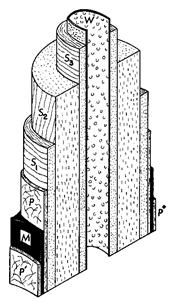
\includegraphics[scale=0.7]{img/ch6_couches}
	\caption{Représentation schématique de la paroi cellulaire chez une trachéide de conifère. M: lamelle moyenne; P et P': paroi primaire; S\sub{1}: couche externe de la paroi secondaire; S\sub{2}: couche médiane de la paroi secondaire; S\sub{3}: couche interne de la paroi secondaire; W : membrane verruqueuse (d'après \cite{choong1997wood}).}
\label{fig:couches}
\end{figure}

\subsection{La lamelle moyenne}

La lamelle moyenne a pour fonction de cimenter les cellules adjacentes. Elle est isotrope et composée de substances amorphes telles que les pectines et la lignine. Les pectines, substances hautement polymérisées, sont sécrétées en quantité importante au cours du cloisonnement cellulaire. La teneur en lignine est faible chez les cellules proches du cambium et elle augmente pour devenir très importante à mesure qu'on s'en éloigne. La faible teneur en lignine de la lamelle moyenne près du cambium permet le développement des cellules du bois, la pectine étant relativement souple. L'épaisseur de la lamelle moyenne varie d'environ 0,2 à 2,0 \micro m.

\subsection{La paroi primaire}

La paroi primaire est la paroi de la cellule vivante en développement dès le méristème secondaire (cambium). La paroi primaire est fine et plastique chez la jeune cellule végétale, ce qui permet son développement à partir du cambium. La paroi primaire ne fait qu'environ 0,1 \micro m. Il est donc difficile, voir même impossible de la voir au microscope optique. On a donc défini la lamelle moyenne composée qui englobe la lamelle moyenne et les parois primaires de deux cellules adjacentes.

La paroi primaire est composée d'un peu de cellulose (9\%), d'hémicelluloses, de pectine, de lignine et d'eau (plus de 70\%), la lignine n'étant présente que chez les cellules matures. On retrouve donc peu de microfibrilles dans cette \og matrice \fg. En fait, elles n'occupent que 2,5 à 5,0\% du volume de la paroi primaire. L'orientation générale des microfibrilles de la paroi primaire est d'environ 85 par rapport à la direction axiale de la cellule.

\subsection{La paroi secondaire}

Une fois que la cellule a atteint sa taille maximale, la paroi \og grandit \fg vers l'intérieur en plusieurs couches: S\sub{1}, S\sub{2} et S\sub{3}. La matrice de lignine et d'hémicelluloses est beaucoup moins importante dans la paroi secondaire, la teneur en cellulose atteignant jusqu'à 94\% de la masse, ce qui confère au bois sa résistance mécanique. L'angle que font les microfibrilles avec la direction axiale des cellules varie pour les trois couches de la paroi secondaire. La croissance de la paroi secondaire serait cyclique, la cellulose étant produite le jour et la lignine la nuit.\\

Les ponctuations des trachéides, fibres et éléments de vaisseaux se mettent en place lors de la croissance de la paroi secondaire. Lorsque ces cellules ont terminé leur développement, le protoplasme (noyau + cytoplasme) meurt, ce qui n'est pas le cas pour les parenchymes qui demeurent en vie jusqu'à ce qu'il y ait duraminisation. Lorsque la paroi secondaire est mature, elle est dense et rigide. Il n'y a donc plus de croissance possible.

\subsection{Structure de la paroi secondaire}

\subsubsection{Couche externe de la paroi secondaire (S\sub{1})}

La couche externe de la paroi secondaire est une couche de transition entre la paroi primaire et la couche médiane de la paroi secondaire (S\sub{2}). Elle est mince (0,1 à 0,2 \micro m) et les microfibrilles y forment une spirale faisant un angle de 50 à 70\textdegree{} par rapport à la direction axiale de la cellule.

\subsubsection{Couche médiane de la paroi secondaire (S\sub{2})}

La couche médiane de la paroi secondaire est la plus importante autant en terme de volume qu'en terme d'impact sur les propriétés du bois. Son épaisseur varie de 1 à 5 \micro m et les microfibrilles y forment une spirale faisant un angle de 10 à 30\textdegree{} par rapport à la direction axiale de la cellule. À cause de cet angle faible des microfibrilles, la couche S\sub{2} change de dimension en épaisseur mais peu en longueur suite à la sorption de l'eau liée. L'angle des microfibrilles est beaucoup plus fort pour le bois juvénile et le bois de réaction que pour le bois adulte normal, ce qui explique la forte tendance au gauchissement de ce type de bois au séchage. L'épaisseur de la couche S\sub{2}  explique la variation de l'épaisseur de la paroi cellulaire entre le bois initial et le bois final.

\subsubsection{Couche interne de la paroi secondaire (S\sub{3})}\label{s3}

La couche interne de la paroi secondaire est mince (0,05 à 0,35 \micro m). Les microfibrilles y forment une spirale faisant un angle de 60 à 90\textdegree{} par rapport à la direction axiale de la cellule.

\subsubsection{Structure des parois cellulaires des parenchymes de xylème}

Il n'y a pas de paroi secondaire chez les parenchymes du xylème. On y retrouve plutôt des parois primaires \og épaissies \fg.\\

La proportion en volume des composantes de la paroi cellulaire est présentée au Tableau \ref{tab:proportionvolume}.

\begin{table}[ht]
\centering
	\begin{tabular}{c c}
	\hline
	\bf Composante & \bf Valeur \\
	\hline
	LMC & 2\% (constant) \\
	S\sub{1} & 10 à 20\% (variable) \\
	S\sub{2} & 68 à 78\% (variable) \\
	S\sub{3} &	8\% (constant) \\
	\hline
	\end{tabular}
\caption{Proportion en volume des composantes de la paroi cellulaire.}
\label{tab:proportionvolume}
\end{table}

\subsection{Distribution des constituants chimiques dans la paroi cellulaire}

La distribution des constituants chimiques dans la paroi cellulaire est présentée à la Figure~\ref{fig:prop}. On remarque que la teneur en lignine est maximale dans la lamelle moyenne composée et diminue vers l'intérieur de la cellule. Inversement, la teneur en cellulose est minimale dans la lamelle moyenne composée, maximale dans la couche S\sub{2} et diminue légèrement dans la couche S\sub{3}. La plus grande quantité de lignine se retrouve dans la couche S\sub{2} car elle est la plus épaisse bien que la teneur en lignine n'y soit pas très élevée.

\begin{figure}[h]
\centering
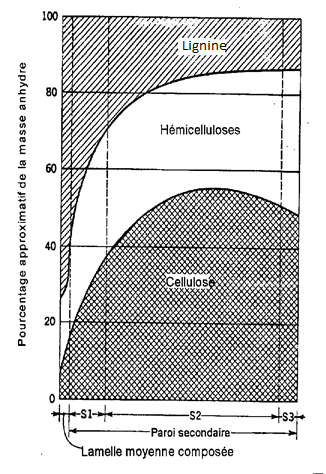
\includegraphics[scale=0.7]{img/ch6_prop}
\caption{Distribution des constituants chimiques de la paroi cellulaire (adapté de \cite{panshin1980textbook}).}
\label{fig:prop}
\end{figure}

\section{Notions complémentaires}

\subsection{Structure des ponctuations}

Les trois principaux types de ponctuations sont présentés à la Figure~\ref{fig:ponctuations2_rep}. On y reconnaît les ponctuations simples que l'on retrouve entre deux cellules de parenchyme, les ponctuations aréolées que l'on retrouve entre deux trachéides, deux éléments de vaisseaux ou deux fibres et les ponctuations semi-aréolées que l'on retrouve entre une cellule de parenchyme et une trachéide, un élément de vaisseau ou une fibre.
\\

Notons également les éléments suivants :

\begin{itemize}
\item le \og margo \fg d'une ponctuation aréolée chez les résineux est un réseau (filet) de paroi primaire flexible (pas de lamelle moyenne);
\item le \og torus \fg d'une ponctuation aréolée chez les résineux est un épaississement de la lamelle moyenne composée;
\item des incrustations se déposent sur le torus et la membrane de la ponctuation, surtout dans le bois de duramen, diminuant ainsi la perméabilité du bois.
\end{itemize}

\begin{figure}[!h]
	\centering
	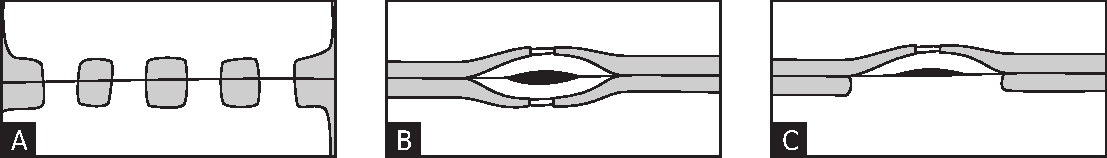
\includegraphics[scale=0.7]{img/ch3_ponctuations2}
	\caption{Trois principaux types de ponctuations. a) ponctuation simple, b) ponctuation aréolée, c) ponctuation semi-aréolée.}
	\label{fig:ponctuations2_rep}
\end{figure}

\subsection{Impact des composantes chimiques sur les propriétés du bois et son utilisation}

\begin{multicols}{2}
\subsubsection{Cellulose}

\begin{itemize}
\item résistance à la traction longitudinale élevée
\item fabrication des pâtes et papiers
\item comportement élastique du bois
\end{itemize}			

\subsubsection{Lignine et hémicelluloses}
	
\begin{itemize}
\item cimentent les cellules et les microfibrilles entre elles
\item résistance mécanique générale du bois
\item comportement plastique du bois
\end{itemize}

\subsubsection{Hygroscopicité du bois}	

\begin{itemize}
\item cellulose (groupements --OH)
\item pectines et hémicelluloses sont hygroscopiques
\end{itemize}

\subsubsection{Gonflement et retrait}\label{gonflement}

\begin{itemize}
\item L < R < T
\item structure du bois
\item angle des microfibrilles dans la couche S\sub{2}
\end{itemize}

\todo{Référez-vous au schéma fait en classe pour expliquer l'effet de l'angle des microfibrilles sur l'ampleur des changements dimensionels dans chaque direction}

\subsubsection{Substances extractibles}
	
\begin{itemize}
\item stabilité dimensionnelle (peu hygroscopiques)
\item relations bois-eau
\item couleur, odeur
\item durabilité
\end{itemize}
\end{multicols}


%Références
%Fengel, D.; Wegener, G. 1989. Wood - chemistry, ultrastructure, reactions. Walter de Gruyter, Berlin. 613 p.
%Panshin, A.J.; de Zeeuw, C. 1980. Textbook of wood technology. Fourth edition. McGraw-Hill Book Co. New York. 722 p.
%Siau, J.F. 1995. Wood: Influence of moisture on physical properties. Department of Wood Science and Forest Products, Virginia Polythechnic Institute and State University. 227 p. 
